\section{Tracing}
\label{sec:tracing}

COMPSs Runtime has a built-in instrumentation system to generate post-execution tracefiles of the applications' execution. The tracefiles contain different events representing the COMPSs master state, the tasks' execution state, and the data transfers (transfers' information is only available when using NIO adaptor), and are useful for both visual and numerical performance analysis and diagnosis. The instrumentation process essentially intercepts and logs different events, so it adds overhead to the execution time of the application.


The tracing system uses Extrae to generate tracefiles of the execution that, in turn, can be visualized with Paraver. Both tools are developed and maintained by the Performance Tools team of the BSC and are available on its web page 
\url{http://www.bsc.es/computer-sciences/performance-tools}. 


For each worker node and the master, Extrae keeps track of the events in an intermediate format file (with \textit{.mpit} extension). At the end of the execution, all intermediate files are gathered and merged with Extrae's \textit{mpi2prv} command in order to create the final tracefile, a Paraver format file (.prv). See the visualization section \ref{sec:Visualization} of this manual for further information about the Paraver tool.


When instrumentation is activated, Extrae outputs several messages corresponding to the tracing initialization, intermediate files' creation, and
the merging process. 


At present time, COMPSs tracing features two execution modes:


\begin{description}
\item [Basic,] aimed at COMPSs applications developers
\item [Advanced,] for COMPSs developers and users with access to its source code or custom installations
\end{description}


Next sections describe the information provided by each mode and how to use them.


\subsection{Basic Mode}

This mode is aimed at COMPSs' apps users and developers. It instruments computing threads and some management resources providing information about tasks' executions, 
data transfers, and hardware counters if PAPI is available (see PAPI counters appendix \ref{sec:papi} for more info). 

\subsubsection{Usage}

In order to activate basic tracing one needs to provide one of the following arguments to the execution command:

\begin{itemize}
 \item -t
 \item --tracing
 \item --tracing=basic
 \item --tracing=true
\end{itemize}


\noindent Examples given:

\begin{lstlisting}[language=bash]
runcompss --tracing application_name application_args
\end{lstlisting}

\noindent Figure \ref{fig:basic_trace} was generated as follows:


\begin{lstlisting}[language=bash]
runcompss \
     --lang=java \
     --tracing \
     --classpath=/path/to/jar/kmeans.jar \
     kmeans.KMeans
\end{lstlisting}

When tracing is activated, Extrae generates additional output to help the user ensure that instrumentation is turned on and working without issues. On basic mode this is the output users should see when tracing is working correctly:

\begin{lstlisting}[language=bash]
*** RUNNING JAVA APPLICATION KMEANS
Resolved: /path/to/jar/kmeans.jar:

----------------- Executing kmeans.Kmeans --------------------------

Extrae: WARNING!
Extrae: WARNING! XML parser version and property 'xml-parser-id' do not match. Check the XML file. Trying to proceed...
Extrae: WARNING!
Extrae: xml-parser-id found 'Id: xml-parse.c 3682 2015-11-26 14:32:27Z harald $' when expecting 'Id: xml-parse.c 3918 2016-03-11 14:59:01Z harald $'.
Welcome to Extrae 3.3.0 (revision 3966 based on extrae/trunk)
Extrae: Parsing the configuration file (/opt/COMPSs/Runtime/scripts/user/../../configuration/xml/tracing/extrae_basic.xml) begins
Extrae: Tracing package is located on /opt/COMPSs/Dependencies/extrae/
Extrae: Generating intermediate files for Paraver traces.
Extrae: Warning! change-at-time time units not specified. Using seconds
Extrae: PAPI domain set to ALL for HWC set 1
Extrae: HWC set 1 contains following counters < PAPI_TOT_INS (0x80000032) PAPI_TOT_CYC (0x8000003b) PAPI_L2_DCM (0x80000002) PAPI_L3_TCM (0x80000008) > - never changes
Extrae: Warning! change-at-time time units not specified. Using seconds
WARNING: IT Properties file is null. Setting default values
[   API]  -  Deploying COMPSs Runtime v1.4 (build 20160412-1147.r2040)
[   API]  -  Tracing is activated
[   API]  -  Starting COMPSs Runtime v1.4 (build 20160412-1147.r2040)
...
...
...
merger: Output trace format is: Paraver
merger: Extrae 3.3.0 (revision 3966 based on extrae/trunk)
mpi2prv: Assigned nodes < Marginis >
mpi2prv: Assigned size per processor < <1 Mbyte >
mpi2prv: File set-0/TRACE@Marginis.0000001904000000000000.mpit is object 1.1.1 on node Marginis assigned to processor 0
mpi2prv: File set-0/TRACE@Marginis.0000001904000000000001.mpit is object 1.1.2 on node Marginis assigned to processor 0
mpi2prv: File set-0/TRACE@Marginis.0000001904000000000002.mpit is object 1.1.3 on node Marginis assigned to processor 0
mpi2prv: File set-0/TRACE@Marginis.0000001980000001000000.mpit is object 1.2.1 on node Marginis assigned to processor 0
mpi2prv: File set-0/TRACE@Marginis.0000001980000001000001.mpit is object 1.2.2 on node Marginis assigned to processor 0
mpi2prv: File set-0/TRACE@Marginis.0000001980000001000002.mpit is object 1.2.3 on node Marginis assigned to processor 0
mpi2prv: File set-0/TRACE@Marginis.0000001980000001000003.mpit is object 1.2.4 on node Marginis assigned to processor 0
mpi2prv: File set-0/TRACE@Marginis.0000001980000001000004.mpit is object 1.2.5 on node Marginis assigned to processor 0
mpi2prv: Time synchronization has been turned off
mpi2prv: A total of 9 symbols were imported from TRACE.sym file
mpi2prv: 0 function symbols imported
mpi2prv: 9 HWC counter descriptions imported
mpi2prv: Checking for target directory existance... exists, ok!
mpi2prv: Selected output trace format is Paraver
mpi2prv: Stored trace format is Paraver
mpi2prv: Searching synchronization points... done
mpi2prv: Time Synchronization disabled.
mpi2prv: Circular buffer enabled at tracing time? NO
mpi2prv: Parsing intermediate files
mpi2prv: Progress 1 of 2 ... 5% 10% 15% 20% 25% 30% 35% 40% 45% 50% 55% 60% 65% 70% 75% 80% 85% 90% 95% done
mpi2prv: Processor 0 succeeded to translate its assigned files
mpi2prv: Elapsed time translating files: 0 hours 0 minutes 0 seconds
mpi2prv: Elapsed time sorting addresses: 0 hours 0 minutes 0 seconds
mpi2prv: Generating tracefile (intermediate buffers of 838848 events)
         This process can take a while. Please, be patient.
mpi2prv: Progress 2 of 2 ... 5% 10% 15% 20% 25% 30% 35% 40% 45% 50% 55% 60% 65% 70% 75% 80% 85% 90% 95% done
mpi2prv: Warning! Clock accuracy seems to be in microseconds instead of nanoseconds.
mpi2prv: Elapsed time merge step: 0 hours 0 minutes 0 seconds
mpi2prv: Resulting tracefile occupies 991743 bytes
mpi2prv: Removing temporal files... done
mpi2prv: Elapsed time removing temporal files: 0 hours 0 minutes 0 seconds
mpi2prv: Congratulations! ./trace/kmeans.Kmeans_compss_trace_1460456106.prv has been generated.
[   API]  -  Execution Finished
Extrae: Tracing buffer can hold 100000 events
Extrae: Circular buffer disabled.
Extrae: Warning! <dynamic-memory> tag will be ignored. This library does support instrumenting dynamic memory calls.
Extrae: Warning! <input-output> tag will be ignored. This library does support instrumenting I/O calls.
Extrae: Dynamic memory instrumentation is disabled.
Extrae: Basic I/O memory instrumentation is disabled.
Extrae: Parsing the configuration file (/opt/COMPSs/Runtime/scripts/user/../../configuration/xml/tracing/extrae_basic.xml) has ended
Extrae: Intermediate traces will be stored in /home/kurtz/compss/tests_local/app10
Extrae: Tracing mode is set to: Detail.
Extrae: Successfully initiated with 1 tasks and 1 threads
\end{lstlisting}

It contains diverse information about the tracing, for example, Extrae version used (3.3.0), the XML configuration file used (extrae\_basic.xml), the amount of 
threads instrumented (objects through 1.1.1 to 1.2.5), available hardware counters ( PAPI\_TOT\_INS (0x80000032) ... PAPI\_L3\_TCM (0x80000008) ) or the name 
of the generated tracefile (./trace/kmeans.Kmeans\_compss\_trace\_1460456106.prv). When using NIO communications adaptor with debug activated, the log of each worker
also contains the Extrae initialization information.



\subsubsection{Instrumented Threads}


Basic traces instrument the following threads:

\begin{itemize}
 \item Master node (3 threads)
 \begin {itemize}
 \item COMPSs runtime
 \item Task Dispatcher
 \item Access Processor
 \end{itemize}
 \item Worker node (1 + Computing Units)
 \begin{itemize}
  \item Main thread
  \item Number of threads available for computing
 \end{itemize}
\end{itemize}

\subsubsection{Information Available}

The basic mode tracefiles contain three kinds of information:

\begin{description}
 \item [Events,] marking diverse situations such as the runtime start, tasks' execution or synchronization points.
 \item [Communications,] showing the transfers and requests of the parameters needed by COMPSs tasks.
 \item [Hardware counters,] of the execution obtained with Performance API (see PAPI counters appendix \ref{sec:papi})
\end{description}


\subsubsection{Trace Example}

Figure \ref{fig:basic_trace} is a tracefile generated by the execution of a k-means clustering algorithm. Each timeline contains information of a 
different resource, and each event's name is on the legend. Depending on the number of computing threads specified for each worker, the number of timelines varies. 
However the following threads are always shown:



\begin{description}
 \item [Master - Thread 1.1.1, ] \hfill \\ this timeline shows the actions performed by the main thread of the COMPSs application
 \item [Task Dispatcher - Thread 1.1.2,] \hfill \\ shows information about the state and scheduling of the tasks to be executed.
 \item [Access Processor - Thread 1.1.3,] \hfill \\  all the events related to the tasks' parameters management, such as dependencies or transfers are shown in this thread.
 \item [Worker X Master - Thread 1.X.1,] \hfill \\ this thread is the master of each worker and handles the computing resources and transfers.  Is is repeated for each available resource. All data events of the worker, such as requests, transfers and receives are marked on this timeline (when using the appropriate configurations).
 \item [Worker X Computing Unit Y - Thread 1.X.Y] \hfill \\ shows the actual tasks execution information and  is repeated as many times as computing threads has the worker X
\end{description}


\begin{landscape}
\begin{figure}[ht!]
  \centering
    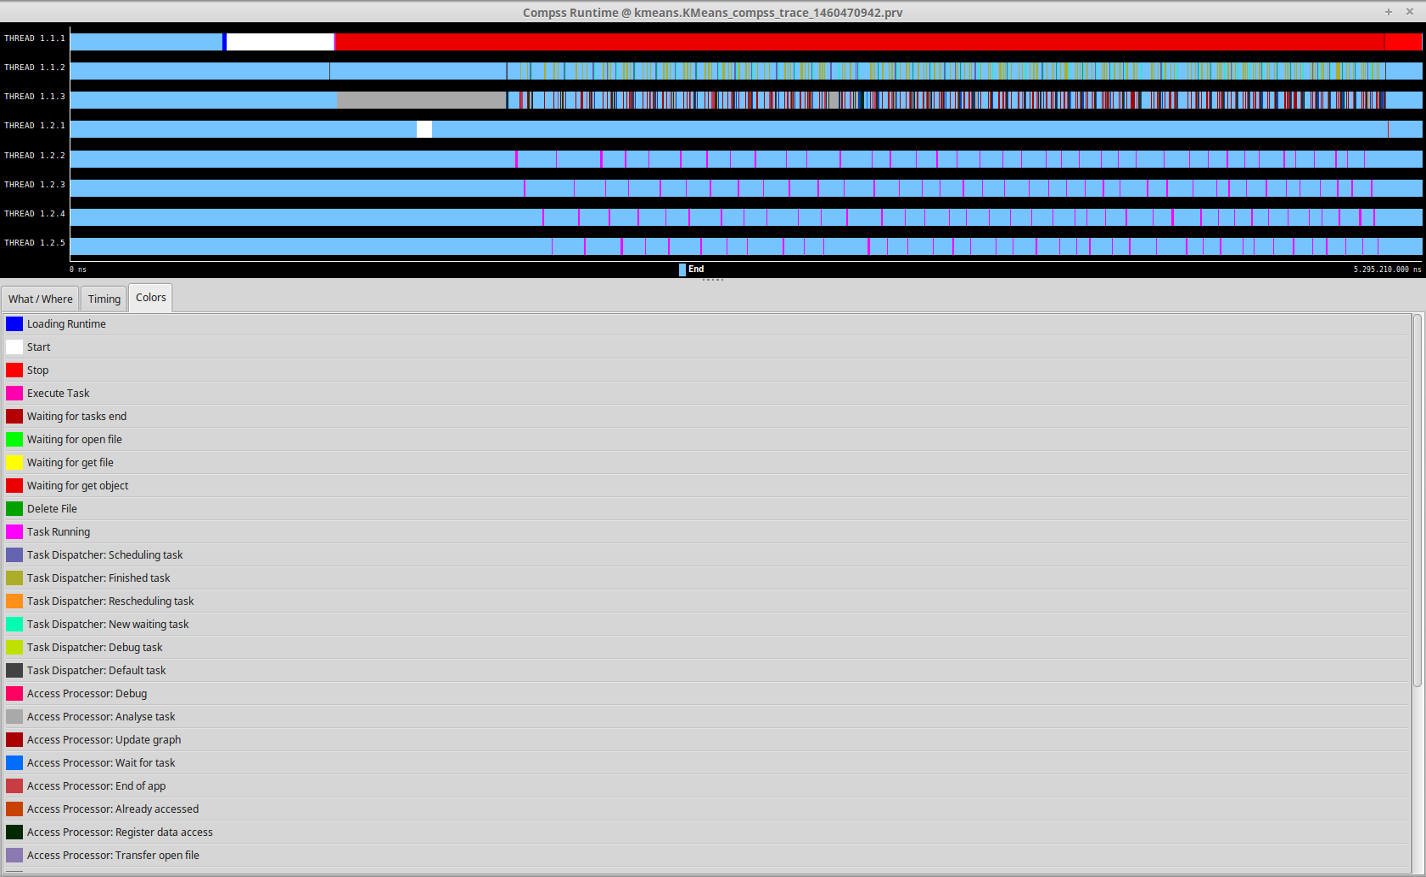
\includegraphics[width=\linewidth]{./Sections/2_Execution/Figures/basic.png}
    \caption{Basic mode tracefile for a k-means algorithm visualized with compss\_runtime.cfg}
    \label{fig:basic_trace}
\end{figure}
\end{landscape}

\subsection{Advanced Mode}
This mode is for more advanced COMPSs' users and developers who want to customize further the information provided by the tracing or need rawer information like pthreads calls or Java garbage collection. With it, every single thread created during the execution is traced.
\\
\\
\textbf{N.B.:} The extra information provided by the advanced mode is only available on the workers when using NIO adaptor.


\subsubsection{Usage}

In order to activate the advanced tracing add the following option to the execution:

\begin{itemize}
 \item --tracing=advanced
\end{itemize}

\noindent Examples given:

\begin{lstlisting}[language=bash]
runcompss --tracing=advanced application_name application_args
\end{lstlisting}

\noindent Figure \ref{fig:advanced_trace} was generated as follows:


\begin{lstlisting}[language=bash]
runcompss \
     --lang=java \
     --tracing=advanced \
     --classpath=/path/to/jar/kmeans.jar \
     kmeans.KMeans
\end{lstlisting}


When advanced tracing is activated, the configuration file reported on the output is \textit{extrae\_advanced.xml}. 

\begin{lstlisting}[language=bash]
*** RUNNING JAVA APPLICATION KMEANS
...
...
...
Welcome to Extrae 3.3.0 (revision 3966 based on extrae/trunk)
Extrae: Parsing the configuration file (/opt/COMPSs/Runtime/scripts/user/../../configuration/xml/tracing/extrae_advanced.xml) begins
\end{lstlisting}

This is the default file used for advanced tracing. However, advanced users can modify it in order to customize the information provided by Extrae. The configuration file is read first by the master on the \textit{runcompss} script. When using NIO adaptor for communication, the configuration file is also read when each worker is started (on \textit{persistent\_worker.sh} or \textit{persistent\_worker\_starter.sh} depending on the execution environment).

If the default file is modified, the changes always affect the master, and also the workers when using NIO. Modifying the scripts which turn on the master and the workers is possible to achieve different instrumentations for master/workers. However, not all Extrae available XML configurations work with COMPSs,
some of them can make the runtime or workers crash so modify them at your discretion and risk. More information about instrumentation XML configurations
on Extrae User Guide at: 
\url{https://www.bsc.es/computer-sciences/performance-tools/trace-generation/extrae/extrae-user-guide}.


\subsubsection{Instrumented Threads}

Advanced mode instruments all the pthreads created during the application execution. It contains all the threads shown on basic traces plus extra ones used to
call command-line commands, I/O streams managers and all actions which create a new process. Due to the temporal nature of many of this threads, they may contain little information or appear just at specific parts of the execution pipeline.

\subsubsection{Information Available}

The advanced mode tracefiles contain the same information as the basic ones:


\begin{description}
 \item [Events,] marking diverse situations such as the runtime start, tasks' execution or synchronization points.
 \item [Communications,] showing the transfers and requests of the parameters needed by COMPSs tasks.
 \item [Hardware counters,] of the execution obtained with Performance API (see PAPI counters appendix \ref{sec:papi})
\end{description}


\subsubsection{Trace Example}

Figure \ref{fig:advanced_trace} shows the total completed instructions for a sample program executed with the advanced tracing mode. Note that the thread - resource correspondence described on the basic trace example is no longer static and thus cannot be inferred. Nonetheless, they can be found thanks to the named events shown in other configurations such as \textit{compss\_runtime.cfg}.


\begin{landscape}
\begin{figure}[ht!]
  \centering
    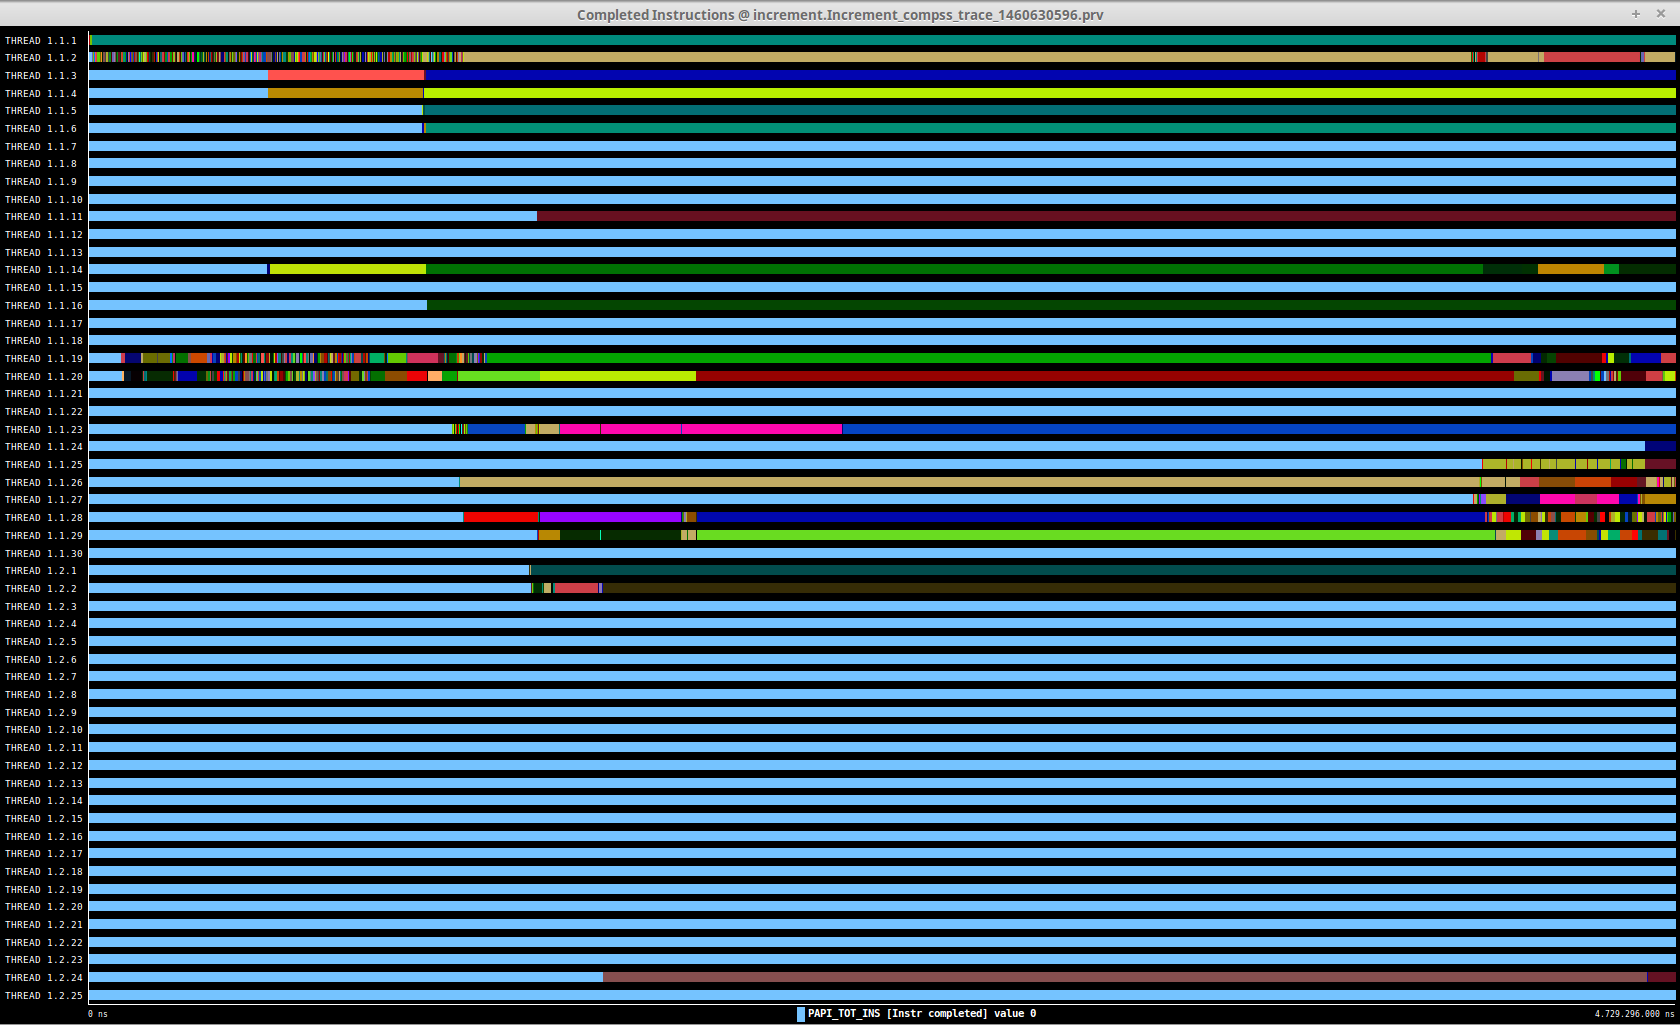
\includegraphics[width=\linewidth]{./Sections/2_Execution/Figures/advanced.png}
    \caption{Advanced mode tracefile for a testing program showing the total completed instructions}
    \label{fig:advanced_trace}
\end{figure}
\end{landscape}

For further information about Extrae, please visit the following site: 
\begin{center}
\url{http://www.bsc.es/computer-science/extrae} 
\end{center}


\subsection{Custom Extrae}

COMPSs uses the environment variable EXTRAE\_HOME to get the reference to its installation directory (by default: \textit{/opt/COMPSs/Dependencies/extrae} ). However, if the variable is already defined once the runtime is started, COMPSs will not override it. User can take advantage of this fact in order to use custom extrae installations. Just set the EXTRAE\_HOME to the directory where your custom package is and make sure that it is also set for the worker's environment. 
\\
\\
Be aware that using different extrae packages can break the runtime and executions so change it at your own risk.